\chapter{
Generating the transformation algebra of a world-agent pair
\draftnote{blue}{V1.5}{}
}
\draftnote{purple}{PS}{
\begin{enumerate}
    \item (visual) Span algorithms across entire page.
    \item (?) Section containing a Step-by-step example of the algorithm.
    \item (Preliminaries) How to read the properties (identity, commutativity, identity, inverse) directly from a Cayley table.
    \item (?) Change the symbol for the set of action functions from $\mathcal{T}$ to $F$ or $\mathcal{F}$ ?
\end{enumerate}
}

The latest version of the code for this chapter can be found at
\begin{center}
    \url{https://github.com/awjdean/CayleyTableGeneration}
\end{center}

%%%%%%%%%%%%%%%%%%%%%%%%%%%%%%%%%%%%%%%%%%%%%
\section{Motivation}

\newthought{To gain an} intuition for the structure of different worlds, to test our theoretical predictions, and to illustrate our theoretical work with examples, we developed an algorithm that uses an agent’s atomic actions to generate the transformation algebra $\hat{A}^{*}/\sim$ of a world-agent pair.

After generating $\hat{A}^{*}/\sim$, we also check the following properties of the algebra algorithmically:
\begin{enumerate}
    \item the presence of identity, including the presence of left and right identity elements separately;
    \item the presence of inverses, including the presence of left and right inverses separately for each element;
    \item associativity;
    \item commutativity; and
    \item the order of each element in the algebra.
\end{enumerate}
We display this structure as a generalised version of a Cayley table \autocite{cayley1854theory}, which is a multiplication table for the distinct elements of the algebra.

%%%%%%%%%%%%%%%%%%%%%%%%%%%%%%%%%%%%%%%%%%%%%
\section{Preliminaries}

We represent the structure of the transformation algebra $(\hat{A}^{*}/\sim, \circ_{\sim})$ for a world-agent pair using a \emph{generalised Cayley table}, which systematically displays the results of combining each pair of elements in the algebra; Cayley tables can be used to characterize the operation of any finite magma.
Formally, the generalised Cayley table $T(S, \star)$ of an algebra $(S, \star)$, which consists of a finite set $S = \{s_{1}, s_{2}, \dots, s_{n}\}$ equipped with a binary operation $\star: S \times S \to S$, is the $n \times n$ matrix where
\begin{enumerate}
    \item the rows and columns are labelled by the elements of $S$;
    \item the entry at the intersection of the row labelled $s_{i}$ and the column labelled $s_{j}$ is
    \begin{equation}
        s_{i} \star s_{j};
    \end{equation}
\end{enumerate}
the generalised Cayley table for $(S, \star)$ is given by
\begin{table}[H]
    \centering
    \begin{tabular}{c|cccc}
        $\star$ & $s_{1}$ & $s_{2}$ & $\dots$ & $s_{n}$  \\
        \hline
        $s_{1}$ & $s_{1} \star s_{1}$ & $s_{1} \star s_{2}$ & $\dots$ & $s_{1} \star s_{n}$ \\
        $s_{2}$ & $s_{2} \star s_{1}$ & $s_{2} \star s_{2}$ & $\dots$ & $s_{2} \star s_{n}$ \\
        $\vdots$ & $\vdots$ & $\vdots$ & $\vdots$ & $\vdots$ \\
        $s_{n}$ & $s_{n} \star s_{1}$ & $s_{n} \star s_{2}$ & $\dots$ & $s_{n} \star s_{n}$
    \end{tabular}
    \caption{
    Example of a Cayley table for the algebra $(S, \star)$.
    }
\end{table}

The Cayley table $T(S, \star)$ of an algebra $(S, \star)$ fully characterises the structure of the algebra, although some properties are not directly conveyed by the Cayley table (e.g., the associativity of $(S, \star)$).

\begin{notation}
    We denote the Cayley table of an algebra $(S, \star)$ by $T(S, \star)$.
    The entry of the Cayley table $T(S, \star)$ found at the intersection of the row labelled $s_{i}$ and the column labelled $s_{j}$ is denoted by $T(S, \star)[s_{i}, s_{j}]$.
\end{notation}

%%%%%%%%%%%%%%%%%%%%%%%%%%%%%%%%%%%%%%%%%%%%%%%
\section{Description}

For our algorithm to successfully generate the complete transformation algebra of a world, the world must contain a finite number of states, the agent must have a finite number of atomic actions, and all the transformations of the world must be due to the actions of the agent.
The algorithm (\cref{alg:GenerateEquivClasses} below) can be split into three parts: (1) the initialisation step, (2) the expansion step, and (3) the termination condition.

\paragraph{Initialisation.}
We begin by initialising the following variables
\begin{enumerate}
    \item the set $\mathcal{E}$ of equivalence classes consisting of
    \begin{enumerate}
        \item the set $L$ of equivalence class representatives as $L = \{ \varepsilon \}$;
        \item the set $E$ of processed actions as $E = \{ \varepsilon \}$; and
        \item the map $\pi_{\sim}: E \to L$ that assigns each processed element in $E$ to its equivalence class representative in $L$ as $\pi_{\sim}(\varepsilon) = \varepsilon$;
    \end{enumerate}
    \item the set $\mathcal{T}$ of distinct action functions $f_{a}: W \to W$ as $\mathcal{T} = \{f_{\varepsilon}\}$, where $f_{\varepsilon}$ is represented by the tuple
    \begin{align}
        f_{\varepsilon} & = (f_{\varepsilon}(w_{1}), f_{\varepsilon}(w_{2}), \dots, f_{\varepsilon}(w_{n}), f_{\varepsilon}(\bot)) \\
        & = (\varepsilon \hat{\ast} w_{1}, \varepsilon \hat{\ast} w_{2}, \dots, \varepsilon \hat{\ast} w_{n}, \varepsilon \hat{\ast} w_{\bot}) \\
        & = (w_{1}, w_{2}, \dots, w_{n}, \bot);
    \end{align}
    \item the map $\rho: L \to \mathcal{T}$ that assigns each equivalence class representative in $L$ to its action function in $\mathcal{T}$ as $\rho(\varepsilon) = f_{\varepsilon}$.
\end{enumerate}


\paragraph{Expansion.}
In each iteration of the expansion step, we search for new distinct actions to create an equivalence class for in $\mathcal{E}$ by (1) generating candidate elements and then (2) test each candidate element for distinctness by checking if their action functions already exist in $\mathcal{T}$.
\begin{enumerate}
    \item \textbf{Generating candidate elements.}
    During each expansion step, we generate a set $A_{C}$ of elements, which are candidate elements for undiscovered equivalence classes, by left composing each atomic action $\hat{a} \in \hat{A}$ with equivalence class representative actions in $L$.
    For every iteration of the expansion step we only need to create candidates by left composing atomic actions in $\hat{A}$ to the actions in $L$ with the greatest length rather than creating candidates using every action in $L$; this is because if the actions in $L$ with the greatest length at the start of an expansion iteration have a length of $n$, then all actions with a length of less than $n$ have already been checked for distinctness (i.e., they will be in the set $E$ of processed actions) because candidate elements are generated at at each expansion iteration by composing them with a single atomic action and so the length of candidate elements increases by one at each iteration.
    We use a filtering function
    \begin{align}
        & \mathcal{L}_{k}: \mathcal{P}(\hat{A}^{*}) \to \mathcal{P}(\hat{A}^{*}) \quad \text{such that} \\
        & \mathcal{L}_{k}(S) = \{ s \in S \mid |s| = k \},
    \end{align}
    where $\mathcal{P}(\hat{A}^{*})$ is the power set of $\hat{A}^{*}$, to obtain a set containing all equivalence class representatives with a length of $k$.
    This means for the expansion step iteration with candidate elements of length $n$, the set $A_{C}$ of candidate elements is given by
    \begin{align}
        A_{C} = \{ \hat{a} \circ l \mid \hat{a} \in \hat{A}, l \in  \mathcal{L}_{n-1}(L)\}.
    \end{align}
    For the first expansion step iteration, we have $L = \{\varepsilon\}$ and so
    \begin{equation}
        A_{C} = \hat{A} \quad \text{for the first expansion step iteration}.
    \end{equation}

    \item \textbf{Testing candidate elements for distinctness.}
    Consider a candidate element $a_{C} \in A_{C}$.
    First we compute a representative tuple for the action function $f_{a_{C}}$ for $a_{C}$ by applying $a_{C}$ to each world state in $W$:
    \begin{align}
        f_{a_{C}} & = (f_{a_{C}}(w_{1}), f_{a_{C}}(w_{2}), \dots, f_{a_{C}}(w_{n}), f_{a_{C}}(\bot)) \\
        & = (a_{C} \hat{\ast} w_{1}, a_{C} \hat{\ast} w_{2}, \dots, a_{C} \hat{\ast} w_{n}, a_{C} \hat{\ast} w_{\bot}).
    \end{align}
    We then check if this action function tuple $f_{a}$ is already stored in $\mathcal{T}$.
    If $f_{a}$ is already in $\mathcal{T}$ then we add $a_{C}$ to the set $E$ of processed actions and update $\pi$ to map $a_{C}$ to the equivalence class representative with the same action function.
    If $f_{a}$ is not in $\mathcal{T}$ then we add $a_{C}$ to $L$ and $E$, add $f_{a}$ to $\mathcal{T}$, and then update $\pi$ to send $a_{C} \mapsto a_{C}$ and update $\rho$ to send $a_{C} \mapsto f_{a_{C}}$ \footnote{
        Since each distinct action $a \in \hat{A}^{*}/\sim$ can be unique characterised by its $f_{a}$ \draftnote{blue}{}{(from \cref{prp:equivalence_equivalence_on_functions})}, the map $\rho$ is bijective.
    }.
\end{enumerate}


\paragraph{Termination.}
The algorithm halts when an expansion iteration produces no successful candidates (i.e., no new distinct action functions are discovered).


%%%%%%%%%%%%%%%%%%%%%%%%%%%%%%%%%%%%%%%%%%%%%
\subsection{Implementation details}

\paragraph{Problem:}
Assessing the equality of actions.
\\\textit{Solution:}
Actions are used in the algorithm and are stored in $L$ and $E$ as tuples of their unique sequences of atomic actions (i.e., the action $a \in \hat{A}^{*}$ is used and stored as $\operatorname{Seq}(a)$); this means to check if two actions are equal we can just compare these tuples.


\paragraph{Problem:}
Composing two actions using the $\circ$ operator.
\\\textit{Solution:}
We define an operator $\operatorname{Combine}$ which combines two atomic action tuples into a single atomic action tuple:
\begin{equation}
    \operatorname{Combine} : \begin{cases}
       \hat{A}^{k} \times \hat{A}^{p} & \to \hat{A}^{k+p}, \\
        \{\varepsilon\} \times \hat{A}^{k} & \to \hat{A}^{k}, \\
        \hat{A}^{k} \times \{\varepsilon\} & \to \hat{A}^{k}
    \end{cases}
\end{equation}
such that
\begin{align}
    & \operatorname{Combine}((\hat{a}_{k}, \; \dots, \; \hat{a}_{1}), \; (\hat{b}_{p}, \; \dots, \; \hat{b}_{1})) = (\hat{a}_{k}, \; \dots, \; \hat{a}_{1}, \; \hat{b}_{p}, \; \dots, \; \hat{b}_{1}) \\
    & \operatorname{Combine}(\varepsilon, \; (\hat{a}_{k}, \; \dots, \; \hat{a}_{1})) = (\hat{a}_{k}, \; \dots, \; \hat{a}_{1}) \\
     & \operatorname{Combine}((\hat{a}_{k}, \; \dots, \; \hat{a}_{1}), \; \varepsilon) = (\hat{a}_{k}, \; \dots, \; \hat{a}_{1}).
\end{align}

Due to the associativity of $\circ$, we have, for any two actions $a, a' \in \hat{A}^{*}$,
\begin{equation}
	a \circ a' = \operatorname{Seq}^{-1}(\operatorname{Combine}(\operatorname{Seq}(a), \; \operatorname{Seq}(a'))).
\end{equation}
But since we represent the elements of $\hat{A}^{*}$ as atomic action tuples throughout our implementation of \cref{alg:GenerateEquivClasses}, we can use
\begin{equation}
	a \circ a' = \operatorname{Combine}(a, \; a').
\end{equation}
in our implementation.


\paragraph{Problem:}
Characterising the world-agent pair $\mathscr{W}$-$\mathscr{A}$.
\\\textit{Solution:}
The set $W$ of world state and the atomic action effect operator $\hat{\ast}$ are sufficient to fully characterise $\mathscr{W}_{\mathscr{A}}$ for any world-agent pair $\mathscr{W}$-$\mathscr{A}$ (\cref{prp:action_world_characterised_by_world_states_and_atomic_action_effect_operator}); in other words,
\begin{equation}
    \mathscr{W}_{\mathscr{A}} := (W, \hat{\ast})
\end{equation}
Since we are considering worlds with only transformations due to the actions of the agent $\mathscr{A}$, we have
\begin{equation}
    \mathscr{W} = \mathscr{W}_{\mathscr{A}};
\end{equation}
therefore,
\begin{equation}
    \mathscr{W} := (W, \hat{\ast}).
\end{equation}
In our implementation we treat $\hat{*}$ as a part of $\mathscr{W}$.


\paragraph{Problem:}
Assessing equality of action functions $f_{a}$.
\\\textit{Solution:}
By definition of the equality of functions from $W$ to $W$, each action function $f_{a}: W \to W$ can be uniquely represented by the tuple
\begin{equation}
    f_{a} = (f_{a}(w_{1}), f_{a}(w_{2}), \dots, f_{a}(w_{n}), f_{a}(\bot))
\end{equation}
where $W = \{ w_{1}, w_{2}, \dots, w_{n}, \bot\}$.
So to assess if two action functions are equal, we compare their representative action function tuples.
We store action functions as their representative tuples in $\mathcal{T}$.


\paragraph{Problem:}
Dealing with undefined actions.
\\\textit{Solution:}
For worlds with undefined actions, the augmentation of $W$ to $W^{\bot}$ and the augmentation of $D_{A}$ to $D_{A}^{\bot}$ account for undefined actions; if the end result of an action sequence is the undefined state $\bot$, then we know that action sequence is undefined.


\paragraph{Problem:}
Calculating the effect of an action a world state.
\\\textit{Solution:}
In algorithm \ref{alg:GenerateActionOutcome}, we need to calculate the effect of applying any action in $\hat{A}^{*}$ that we come across to any world state $w \in W$.
To avoid having to program in the (indefinitely many) labelled transformations in $D_{A}^{\bot}$ into our implementation of the world $\mathscr{W}$, instead of applying $a$ directly to $w$, we exploit the actions' expressions as their unique sequences of atomic actions to apply each of their constituent atomic actions in order to obtain the resulting world state:
\begin{equation}
\begin{aligned}
    a * w = & \; (\hat{a}_{n} \circ \dots \circ \hat{a}_{2} \circ \hat{a}_{1}) * w \\
    = & \; \hat{a}_{n} * ( \dots (\hat{a}_{2} * (\hat{a}_{1} * w)) \dots);
\end{aligned}
\end{equation}
this is possible because we store actions in $L$ and $E$ as tuples of their unique sequences of atomic actions.


%%%%%%%%%%%%%%%%%%%%%%%%%%%%%%%%%%%%%%%%%%%%%
\section{Pseudocode}

\begin{table*}[htbp]
  \begin{fullwidth}
    \centering
    \begin{tabularx}{\linewidth}{lX}
      \toprule
      \textbf{Notation}                    & \textbf{Description} \\
      \midrule
      $\hat{A}$                          & The set of atomic actions of the agent.
      Elements of $\hat{A}$ are denoted with a $\hat{\ }$. \\
      $\mathscr{W} = (W, \; \hat{\ast})$ & The world characterised by a set $W$ of world states and an atomic action effect map $\hat{\ast}$. \\
      $W$                                & The set of world states. \\
      $\hat{\ast}$                       & The atomic action effect operator $\hat{A} \times W \to W$ that sends an atomic action-world state pair to the resultant world state after the agent performs that atomic action in the world state. \\
      $L$                                & The set of equivalence class representatives. \\
      $E$                                & The set of processed actions. \\
      $\pi$                              & A map $E \to L$ that sends each processed action to its equivalence class representative. \\
      $\mathcal{E} = (L, \; E, \; \pi)$  & The equivalence classes. \\
      $\mathcal{T}$                      & The set of action functions $f_{a}: W \to W$. \\
      $\rho$                             & A map $L \to \mathcal{T}$ that sends each equivalence class representative to its action function. \\
      $n$                                & A loop counter that represents both the number of the current expansion step iteration and the length of the candidate elements being checked in the current expansion step iteration. \\
      $N_{L}$                            & The number of equivalence classes discovered in the previous expansion step iteration. \\
      $A_{C}$                            & The set of elements that are candidates in the current expansion step iteration for undiscovered equivalence classes. \\
      $\mathcal{L}_{k}(S)$               & A filtering function $\mathcal{L}_{k}: \mathcal{P}(\hat{A}^{*}) \to \mathcal{P}(\hat{A}^{*})$ such that $\mathcal{L}_{k}(S) = \{ s \in S \mid |s| = k \}$. \\
      $\operatorname{Combine}$           & The combine operator that composes two action sequences by combining their tuples of atomic actions. \\
      $T(\hat{A}^{*}/\sim, \circ_{\sim})$               & The Cayley table.\\
      \bottomrule
    \end{tabularx}
    \caption{Key for pseudocode.}
  \end{fullwidth}
\end{table*}


%%%%%%%%%%%%%%%%%%%%%%%%%%%%%%%%%%%%%%%%%%%%%
\subsection{Generating the equivalence classes}

\begin{algorithm}[H]
\begin{fullwidth}
\caption{
Generate the equivalence classes $\mathcal{E} = (L, \; E, \; \pi: E \to L)$ for $\sim$ on $\hat{A}^{*}$ and the set of action functions $\mathcal{T} = \{f_{l}: W \to W\}$, where $l \in L$, for a world-agent pair $\mathscr{W}$-$\mathscr{A}$ with a set $\hat{A}$ of atomic actions and $\mathscr{W} = (W, \; \hat{\ast})$.
}
\label{alg:GenerateEquivClasses}
\hrulefill
\begin{algorithmic}[1]
    \Function{GenerateEquivClasses}{$\hat{A}$, \; $\mathscr{W}$}
    \Statex \Comment{Initialise equivalence classes object $\mathcal{E}$.}
    \State $L \gets \{\varepsilon\}$
    \State $E \gets \{\varepsilon\}$
    \State $\pi \gets (\varepsilon \mapsto \varepsilon)$
    \State $\mathcal{E} \gets (L, \; E, \; \pi)$.

    \Statex \Comment{Initialise $\mathcal{T}$ and $\rho$}
    \State $\mathcal{T} \gets \{f_{\varepsilon}\}$
    \State $\rho \gets (\varepsilon \mapsto f_{\varepsilon})$

    \Statex \Comment{Iteratively create candidate action sequences for equivalence class representative elements then check if they are successful candidates.}
    \State $n = 0$
    \State $N_{L} \gets -1$
    \Statex \Comment{If no new distinct equivalence classes found in an expansion step, then halt the algorithm.}
    \While{$N_{L} \neq |L|$}
    \State $n \gets n + 1$
    \State $N_{L} \gets |L|$
    \State $A_{C} \gets \Call{GenerateCandidates}{\mathcal{L}_{n-1}(L), \;  \hat{A}}$

    \For{\textbf{each} $a_{C} \in A_{C}$}
    \State $(\mathcal{E}, \; \mathcal{T}, \; \rho) \gets$ \Call{ProcessCandidate}{$a_{C}$, \; $\mathcal{T}$, \; $\rho$, \; $\mathcal{E}$, \; $\mathscr{W}$}
    \EndFor
    \EndWhile
    \State \Return $\mathcal{E}, \; \mathcal{T}$, \; $\rho$
    \EndFunction
\end{algorithmic}
\end{fullwidth}
\end{algorithm}


\begin{algorithm}[H]
\begin{fullwidth}
\caption{
    Generate new action sequences that are candidates for equivalence class labelling elements.
}
\hrulefill
\begin{algorithmic}[1]
    \Function{GenerateCandidates}{$L$, \;  $\hat{A}$}
    \State $A_{C} \gets \emptyset$
    \ForAll{$(\hat{a}, \; l) \in \hat{A} \times L$}
    \State $a' \gets \operatorname{Combine}(\hat{a}, \; l)$
    \State $A_{C} \gets A_{C} \cup \{a'\}$
    \EndFor
    \State \Return $A_{C}$
    \EndFunction
\end{algorithmic}
\end{fullwidth}
\end{algorithm}


\begin{algorithm}[H]
\begin{fullwidth}
\caption{
    Processes a candidate $a_{C}$ for being an element of an undiscovered equivalence class.
    If $a_{C}$ is a successful candidate, then create a new equivalence classes labelled by $a_{C}$.
    If $a_{C}$ is found to be in another equivalence class then add it to that equivalence class.
}
\hrulefill
\begin{algorithmic}[1]
    \Function{ProcessCandidate}{$a_{C}$, \; $\mathcal{T}$, \; $\rho$, \; $\mathcal{E}$, \; $\mathscr{W}$}
    \State $f_{a_{C}} = \Call{ComputeActionFunction}{a_{C}, \; \mathscr{W}}$

    \If{$f_{a_{C}} \in \mathcal{T}$}
    \Statex \Comment{Add $a_{C}$ to equivalence class in $\mathcal{E}$ with class label that has the same action function $f_{a_{C}}$.}
    \State $\mathcal{E} \gets (\; L, \; E \cup \{a_{C}\}, \; \pi \cup \pi' \;)$, where $\pi': \{a_{C}\} \to L$ such that $\pi'(a_{C}) = \rho^{-1}(f_{a_{C}})$.
    \Else
    \Statex \Comment{Create new equivalence class in $\mathcal{E}$ labelled by $a_{C}$.}
    \State $\mathcal{E}' \gets (\; L \cup \{a_{C}\}, \; E \cup \{a_{C}\}, \; \pi \cup \pi' \;)$, where $\pi': \{a_{C}\} \to \{a_{C}\}$ such that $\pi'(a_{C}) = a_{C}$.

    \Statex \Comment{Add $f_{a_{C}}$ to $\mathcal{T}$.}
    \State $\mathcal{T}' \gets \mathcal{T} \cup \{f_{a_{C}}\}$

    \Statex \Comment{Update $\rho$ to send $a_{C}$ to $f_{a_{C}}$.}
    \State $\rho' \gets \rho \cup \rho''$ where $\rho'': \{a_{C}\} \to \{f_{a_{C}}\}$ such that $\rho''(a_{C}) = f_{a_{C}}$.
    \EndIf
    \State \Return $(\mathcal{E}', \; \mathcal{T}', \; \rho')$
    \EndFunction
\end{algorithmic}
\end{fullwidth}
\end{algorithm}


\begin{algorithm}[H]
\begin{fullwidth}
\caption{
Compute the action function $f_{a}: W \to W$ that sends $w \mapsto a \ast w$.
}
\label{alg:ComputeActionFunction}
\hrulefill
\begin{algorithmic}[1]
    \Function{ComputeActionFunction}{$a$, \; $\mathscr{W}$}
    \State $f_{a} \gets (\emptyset \to \emptyset)$
    \ForAll{$w \in W$}
    \State $w_{a} \gets$ \Call{GenerateActionOutcome}{$a$, \; $w$, \; $\hat{\ast}$}
    \State $f_{a} \gets f_{a} \cup f_{a}'$ where $f_{a}': \{w\} \to \{w_{a}\}$ such that $f_{a}'(w) = w_{a}$
    \EndFor
    \State \Return $f_{a}$
    \EndFunction
\end{algorithmic}
\end{fullwidth}
\end{algorithm}


\begin{algorithm}[H]
\begin{fullwidth}
\caption{
    Generate the outcome state of a world $\mathscr{W}$ when an action sequence $a$ is applied to the world in an initial state $w$.
}
\label{alg:GenerateActionOutcome}
\hrulefill
\begin{algorithmic}[1]
    \Function{GenerateActionOutcome}{$a$, \; $w$, \; $\hat{\ast}$}
    \State $w_{a} \gets w$
    \For{$i \gets 1, \; \dots \;, \; n$}
    \State $w_{a} \gets \hat{a}_{i} \; \hat{\ast} \; w_{a}$ where $\operatorname{Seq}(a) = (\hat{a}_n, \; \hat{a}_{n-1}, \; \dots \;, \; \hat{a}_1)$
    \EndFor
    \State \Return $w_{a}$
    \EndFunction
\end{algorithmic}
\end{fullwidth}
\end{algorithm}


%%%%%%%%%%%%%%%%%%%%%%%%%%%%%%%%%%%%%%%%%%%%%
\subsection{Generating the Cayley table}

\begin{algorithm}[H]
\begin{fullwidth}
\caption{
    Generates the Cayley table $T(\hat{A}^{*}/\sim, \circ_{\sim})$.
}
\label{alg:GenerateCayley}
\hrulefill
\begin{algorithmic}[1]
    \Procedure{GenerateCayley}{$\mathcal{E}$}
    \State $T_{A} \gets$ Empty $|L| \times |L|$ matrix with rows and columns labelled by the elements of $L$.
    \Statex \Comment{Fill actions Cayley table.}
    \For{\textbf{each} $l_{i} \in L$}
    \For{\textbf{each} $l_{j} \in L$}
    \Statex \Comment{Get action function for the combined element.}
    \State $f_{(l_{i} \; \circ \; l_{j})} \gets$ \Call{ComputeCompositionActionFunction}{$l_{i}$, \; $l_{j}$, \; $\mathcal{T}$, \; $\rho$}
    \Statex \Comment{Get equivalence class representative element for the action function $f_{(l_{i} \; \circ \; l_{j})}$ and assign it to the relevant Cayley table entry.}
    \State $T_{A}[l_{i}, l_{j}] \gets \rho^{-1}(f_{(l_{i} \; \circ \; l_{j})})$
    \Statex \Comment{Add $a$ to the equivalence class as $\operatorname{Combine}(l_{i}, l_{j})$.}
    \If{$\operatorname{Combine}(l_{i}, \; l_{j}) \centernot\in E$}
        \State $a \gets \operatorname{Combine}(l_{i}, \; l_{j})$
        \State $\mathcal{E} \gets (\; L, \; E \cup \{a\}, \; \pi \cup \pi' \;)$, where $\pi': \{a\} \to L$ such that $\pi'(a) = \rho^{-1}(f_{(l_{i} \; \circ \; l_{j})})$.
    \EndIf
    \EndFor
    \EndFor
    \State \Return $T_{A}$, $\mathcal{E}$
    \EndProcedure
\end{algorithmic}
\end{fullwidth}
\end{algorithm}


\begin{algorithm}[H]
\begin{fullwidth}
\caption{
    Compute the action function for the combination $l_{L} \circ l_{R}$ of two actions by combining their action functions.
}
\hrulefill
\begin{algorithmic}[1]
    \Procedure{ComputeCompositionActionFunction}{$l_{L}$, \; $l_{R}$, \; $\mathcal{T}$, \; $\rho$}
    \Statex \Comment{Get action functions for $l_{L}$ and $l_{R}$.}
    \State $f_{L} \gets \rho(l_{L})$
    \State $f_{R} \gets \rho(l_{R})$
    
    \State $f_{a} \gets (\emptyset \to \emptyset)$
    \Statex \Comment{Compute the combined action function $f_{a}$}
    \State $f_{a} \gets (\emptyset \to \emptyset)$
    \ForAll{$w_{R, \; I} \in \operatorname{Dom}(f_{R})$}
    \State $w_{R, \; F} \gets f_{R}(w_{R, \; I})$
    \ForAll{$w_{L, \; I} \in \operatorname{Dom}(f_{L})$}
    \If{$w_{L, \; I} = w_{R, \; F}$}
    \State $w_{L, \; F} \gets f_{L}(w_{L, \; I})$
    \State $f_{a} \gets f_{a} \cup f_{a}'$ where $f_{a}': \{w_{R, \; I}\} \to \{w_{L, \; F}\}$ such that $f_{a}'(w_{R, \; I}) = w_{L, \; F}$
    \EndIf
    \EndFor
    \EndFor
    \State \Return $f_{a}$
    \EndProcedure
\end{algorithmic}
\end{fullwidth}
\end{algorithm}

%%%%%%%%%%%%%%%%%%%%%%%%%%%%%%%%%%%%%%%%%%%%%
\section{
Analysis
}

\paragraph{Halting of \cref{alg:GenerateEquivClasses}.}

\begin{propositionE}
    \Cref{alg:GenerateEquivClasses} always halts for finite $W$.
\end{propositionE}
\begin{proofE}
\begin{enumerate}
    \item \textbf{$|L|$ increases monotonically until its final iteration.}
    During each expansion iteration, the set $L$ either grows or remains the same.
    So at each expansion iteration, with a new distinct action is discovered and added to $L$ or no new distinct actions are discovered and the algorithm halts.

    \item \textbf{Upper bound on $|L|$.}
    For a world with $|W|$ world states there are at most $(|W| + 1)^{(|W| + 1)}$ distinct transformations $W^{\bot} \to W^{\bot}$.
    Therefore, the set $L$ can have at most $(|W| + 1)^{(|W| + 1)}$ elements.

    \item \textbf{Halting.}
    If $L$ stops growing for one expansion iteration, then the algorithm halts.
    If $|L| = (|W| + 1)^{(|W| + 1)}$, then there are no more unique action functions and therefore no more distinct actions under $\sim$ and so \cref{alg:GenerateEquivClasses} halts.
    Since $|L|$ increases monotonically when it changes, either $|L|$ reaches $(|W| + 1)^{(|W| + 1)}$ and halts or the algorithm halts before $|L| = (|W| + 1)^{(|W| + 1)}$.
\end{enumerate}
\end{proofE}

While \cref{alg:GenerateEquivClasses} is running, $L$ is a subset of $\hat{A}^{*}/\sim$.
When \cref{alg:GenerateEquivClasses} halts $L = \hat{A}^{*}/\sim$ and $\mathcal{T} = \mathcal{T}_{\hat{A}^{*}/\sim}$ is the complete monoid of action functions\footnote{
When \cref{alg:GenerateEquivClasses} halts, the equivalence classes $\mathcal{E}$ are not complete since there are an infinite number of elements in $\hat{A}^{*}$.
}.

\begin{propositionE}
    When \cref{alg:GenerateEquivClasses} halts, the set $L$ contains all distinct actions under $\sim$ in $\hat{A}^{*}$; in other words, upon halting
    \begin{equation}
        L = \hat{A}^{*}/\sim.
    \end{equation}
\end{propositionE}
\begin{proofE}
\textbf{Proof by contradiction.}
\begin{enumerate}
    \item \textbf{Set up.}
    Assume \cref{alg:GenerateEquivClasses} halts with a set $L$ of discovered distinct actions, but that there exists at least one distinct transformation that is not represented in $L$.
    Let $b$ be the shortest undiscovered distinct action.

    \item \textbf{Decomposition of $b$.}
    We can write $b$ as $b = \hat{a} \circ b'$ where $\hat{a} \in \hat{A}/\sim$ and $b' \in \hat{A}^{*}$.
    Since $b$ is the shortest undiscovered distinct action, either $b'$ must have been discovered and be represented in $L$ or $b'$ is not discovered and $b$ is not the shortest undiscovered distinct action, since $b'$ is shorter than $b$, which is a contradiction.

    \item \textbf{Contradiction.}
    Given that $b'$ is known and represented in $L$, \cref{alg:GenerateEquivClasses} will have left composed $b'$ with every distinct atomic action in $\hat{A}/\sim$, including $\hat{a}$.
    Therefore, \cref{alg:GenerateEquivClasses} must have discovered $b = \hat{a} \circ b'$, which is a contradiction.
\end{enumerate}
\end{proofE}


%%%%%%%%%%%%%%%%%%%%%%%%%%%%%%%%%%%%%%%%%%%%%
\paragraph{Complexity analysis}
Let $|W| = n$ (so $|W^{\bot}| = n+1$) and let $|\hat{A}/\sim| = m$.
In the worst case, \cref{alg:GenerateEquivClasses} must discover all $|W^{\bot}|^{|W^{\bot}|}$ functions $W^{\bot} \to W^{\bot}$.
The algorithm generates new candidate actions by composing discovered distinct actions in $L$ with atomic actions in $\hat{A}$; in the worst case scenario that would mean $m (n+1)^{(n+1)}$ candidate elements to check.
Checking each candidate element costs at least $\mathcal{O}(n)$ time because the the action function for each candidate must be determined for each of the $|W^{\bot}|$ states.
Therefore, an upper bound on the time complexity of \cref{alg:GenerateEquivClasses} is
\begin{equation}
    \mathcal{O}(m \cdot (n+1)^{(n+1)} \cdot n).
\end{equation}

%%%%%%%%%%%%%%%%%%%%%%%%%%%%%%%%%%%%%%%%%%%%%
\paragraph{
Interpretation of \cref{alg:GenerateEquivClasses} as an agent's inference process.
}
\draftnote{blue}{To do}{
\begin{enumerate}
    \item Ideal sensors + perfect inference process.
\end{enumerate}
}
We can interpret our algorithm as the inference process for an agent with ideal sensors and a perfect inference process.



%%%%%%%%%%%%%%%%%%%%%%%%%%%%%%%%%%%%%%%%%%%%%
\whendraft{
\section{Atomic actions affect the transformation algebra \draftnote{blue}{To do}{V0.0}}
\draftnote{blue}{To do}{
\begin{enumerate}
    \item Have a world $\mathscr{W}$ with loads of transformations, then have different agent actions (different labelling map).
    \item Show that it's possible to change the agent but produce the same transformation algebra (e.g., remove $a_{U}$ from $\hat{A}$).
\end{enumerate}
}


We will now explicitly prove that changing the agent can change the transformation algebra $\hat{A}^{*}/\sim$ under $\sim$.
Recall that an agent $\mathscr{A}$ in our framework consists of a set $\hat{A}$ of atomic actions, a representation $\mathscr{Z}$, an observation process $b$, and an inference process $h$.
Consider two agents $\mathscr{A}_{1}$ and $\mathscr{A}_{2}$ each in a copy of our example world $\mathscr{W}_{\alpha}$.
$\mathscr{A}_{1}$ and $\mathscr{A}_{2}$ both have ideal sensors and the inference process $b$ of our agents is \cref{alg:GenerateEquivClasses}.

\begin{figure}[H]
  \centering
    \begin{subfigure}[b]{0.45\linewidth}
        \centering
        \includegraphics[width=\linewidth]{}
        \caption{
        $\hat{\mathscr{W}}_{\mathscr{A}}$ for the world-agent pair $\mathscr{W}_{\alpha}$-$\mathscr{A}_{1}$ with $\hat{A} = \{ a_{1}, a_{R}, a_{L}, a_{U}, a_{D} \}$.
        }
    \end{subfigure}
    \begin{subfigure}[b]{0.45\linewidth}
        \centering
        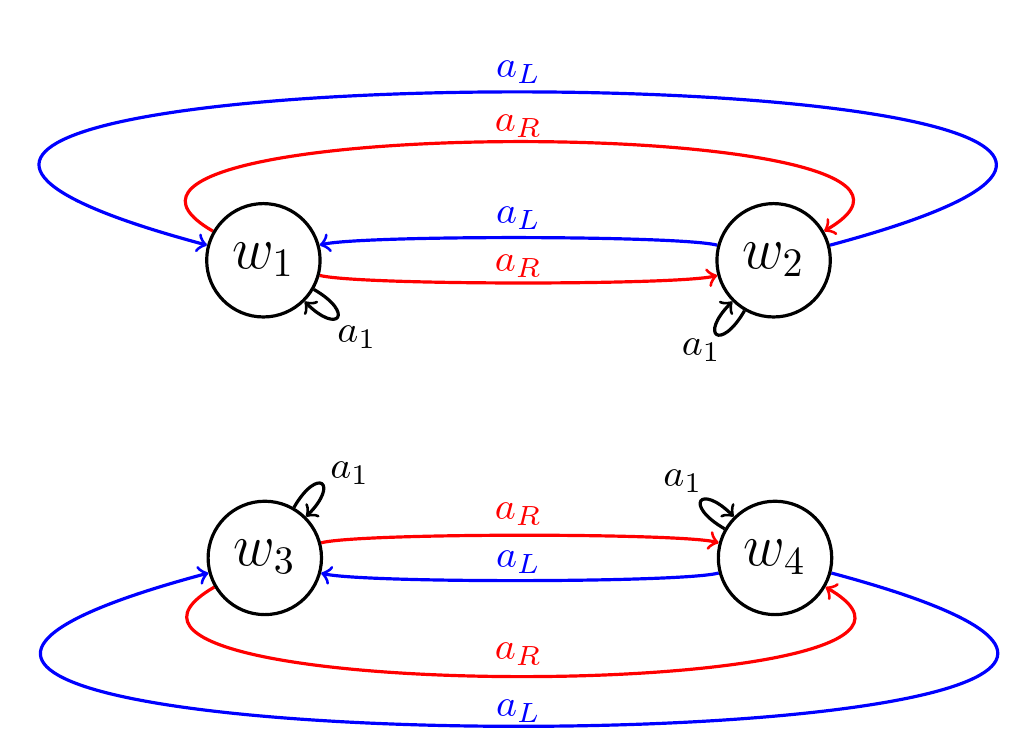
\includegraphics[width=\linewidth]{3Algorithm/Images/action_affect_algebra.png}
        \caption{
        $\hat{\mathscr{W}}_{\mathscr{A}}$ for the world-agent pair $\mathscr{W}_{\alpha}$-$\mathscr{A}_{2}$ with $\hat{A} = \{ a_{1}, a_{R}, a_{L} \}$.
        }
    \end{subfigure}
  \caption{
  \draftnote{blue}{To do}{}
  }
\label{fig:2x2_cyclical_grid_world_wall_states}
\end{figure}

\begin{figure}[H]
    \centering
    \begin{tikzpicture}
        \node (left) {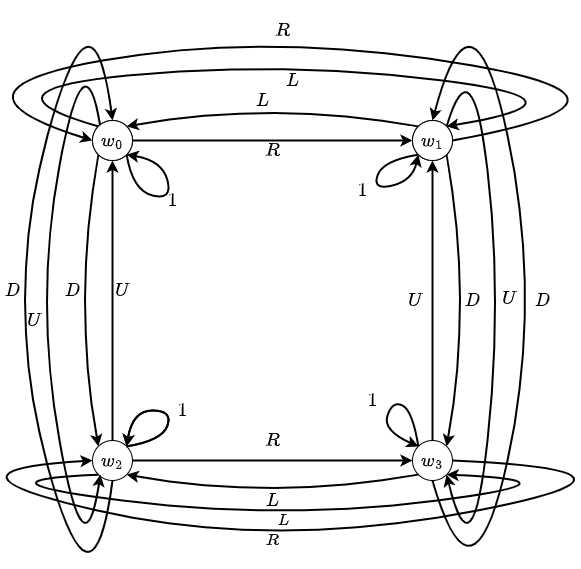
\includegraphics[width=0.6\textwidth]{2MathematicalFramework/Images/2x2-cyclical-min-actions.drawio.png}};
        \node (sim) [right=1cm of left] {};
        \node (right) [right=1cm of sim] {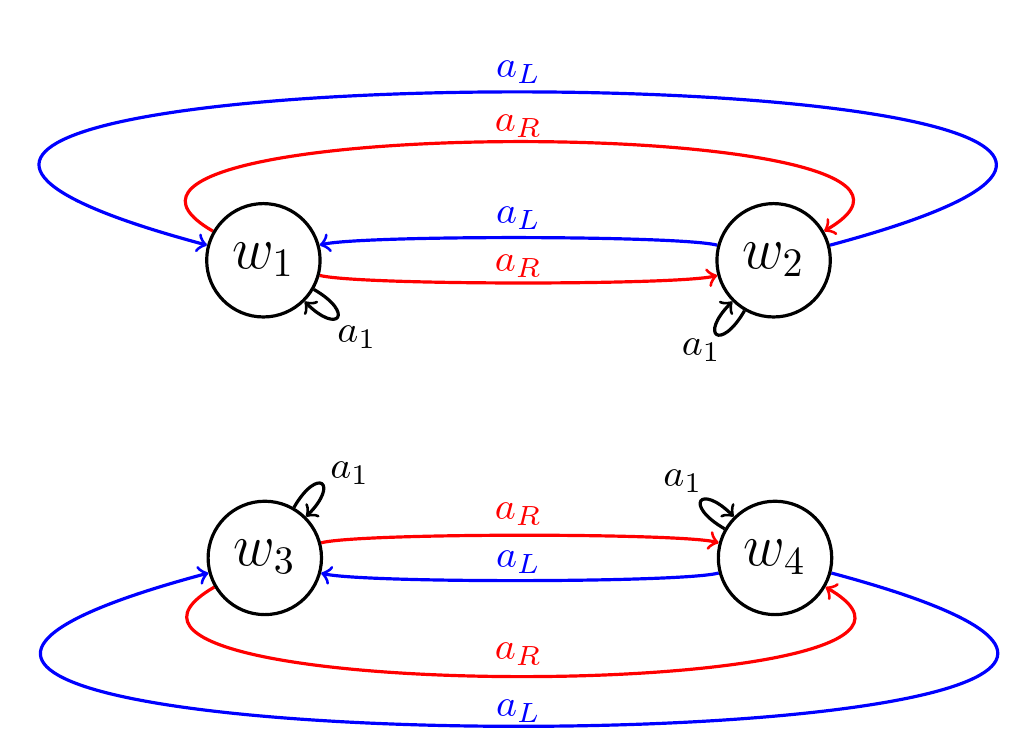
\includegraphics[width=0.6\textwidth]{3Algorithm/Images/action_affect_algebra.png}};
    \end{tikzpicture}
    \caption{
    World diagram showing how $\hat{l}$ labels the atomic action transformations and the trivial transformations of $\mathscr{W}_{\alpha}$-$\mathscr{A}$.
    }
    \label{fig:2x2_cyclical_labelling_with_min_actions}
\end{figure}



Using \cref{alg:GenerateEquivClasses,alg:GenerateCayley} to generate the Cayley tables of $\hat{A}^{*}/\sim$ for $\mathscr{A}_{1}$ and $\mathscr{A}_{2}$ we get the following:
\begin{table}[H]
    \centering
    \begin{tabular}{cc}
        \subcaptionbox{$w_{0}$\label{tab:W_alpha_local_w0_cayley}}{
            \draftnote{blue}{Insert Cayley table for $\mathscr{W}_{A}$ with $\mathscr{A}_{1}$}{}.
        } &
        \subcaptionbox{$w_{1}$}{
            \draftnote{blue}{Insert Cayley table for $\mathscr{W}_{A}$ with $\mathscr{A}_{2}$}{}.
        }
    \end{tabular}
    \caption{
    \draftnote{blue}{To do}{}
    }
    \label{tab:W_alpha_local_cayley_tables}
\end{table}


\draftnote{blue}{Perfect sensors}{
\begin{enumerate}
    \item Definitely want representation $\mathscr{Z}$ to be homomorphic to $\mathscr{W}_{A}$.
    Do we want $\mathscr{Z}$ to be isomorphic to $\mathscr{W}_{A}$ ?
\end{enumerate}
}
}